\documentclass[11pt]{article}

% --- Packages ---
\usepackage[margin=1in]{geometry}
\usepackage{graphicx}
\usepackage{booktabs}
\usepackage{amsmath,amssymb}
\usepackage{natbib}
\usepackage{hyperref}
\usepackage{xcolor}
\usepackage{multirow}
\usepackage{caption}
\usepackage{subcaption}

\hypersetup{
  colorlinks=true,
  linkcolor=blue!60!black,
  citecolor=blue!60!black,
  urlcolor=blue!60!black
}

% --- Figures path ---
\graphicspath{{figures/}}

% --- Title ---
\title{World Properties without World Models:\\
  Recovering Spatial and Temporal Structure from Co-occurrence Statistics in Static Word Embeddings}

\author{
  Elan Barenholtz \\
  \textit{Department of Psychology \& Center for Complex Systems and Brain Sciences} \\
  \textit{Florida Atlantic University} \\
  \texttt{elan.barenholtz@fau.edu}
}

\date{}

\begin{document}
\maketitle

% ============================================================
% ABSTRACT
% ============================================================
\begin{abstract}
Recent work reports that linear probes recover geographic coordinates and historical dates from the hidden states of large language models, interpreting these results as evidence that LLMs learn structured internal ``world models.'' 
We demonstrate that comparable spatial and temporal signals are recoverable from static word embeddings (GloVe and Word2Vec), whose representations are direct functions of co-occurrence statistics. 
Ridge regression probes applied to 300-dimensional embeddings of 100 world cities predict latitude ($R^2 = 0.71$), longitude ($R^2 = 0.78$), and mean annual temperature ($R^2 = 0.47$--$0.62$), despite the absence of contextual processing. 
Probes on 194 historical figures predict birth year with $R^2 = 0.48$--$0.52$. 
Semantic similarity analyses confirm that the geographic signal is interpretable: cosine similarity to climate, directional, and geopolitical vocabulary correlates systematically with latitude and temperature.
These findings indicate that the spatial and temporal structure observed in LLM representations is consistent with distributional statistics inherited from the training corpus, reducing the evidential force of linear decodability as support for emergent world models.
\end{abstract}

% ============================================================
% 1. INTRODUCTION
% ============================================================
\section{Introduction}

Large language models (LLMs) have achieved strong performance across a wide range of domains, including tasks that plausibly require structured knowledge of entities, space, and time.
This empirical success has renewed debates about what types of internal representations such systems acquire, and in particular whether next-token prediction yields structured ``world-model''-like representations or instead exploits high-dimensional regularities in linguistic co-occurrence.
A prominent and empirically concrete strand of evidence in this debate comes from probing: recent work reports that linear probes recover geographic coordinates and historical dates from LLM hidden states, interpreting such linear accessibility as support for linearly organized spatial and temporal representations (and, by extension, world models) \citep{gurnee2023language,touvron2023llama}.

Here we test a simpler alternative explanation.
Specifically, we ask whether the linear recoverability of spatial and temporal properties requires the representational capacity of an LLM, or whether comparable signals are already recoverable from static distributional representations.
To this end, we apply the same probing methodology to GloVe \citep{pennington2014glove} and Word2Vec \citep{mikolov2013efficient}, static word embeddings that are direct functions of co-occurrence statistics and lack contextual processing.

We find that ridge regression probes recover substantial geographic and historical signal from these static embeddings, and that the signal is mediated by graded co-occurrence with semantically interpretable vocabularies (e.g., climate and geopolitical terms).
These results constrain the interpretation of probe-based recoverability: linear decodability alone does not distinguish structured internal modeling from inherited distributional gradients.
Accordingly, claims that probe-based results provide positive evidence for world models should be evaluated against distributional baselines.

\paragraph{Contributions.}
(i) We quantify the extent to which geographic and temporal variables are linearly predictable from static embeddings, providing a distributional baseline for probe-based claims.
(ii) We provide interpretive evidence via semantic similarity analyses showing that the recovered signal tracks graded co-occurrence with climate, directional, and geopolitical vocabulary.


\section{Related Work}

\paragraph{Probe-based evidence for world-structured representations.}
A growing literature uses probing to assess whether language model representations support prediction of geographic, temporal, and other externally grounded attributes \citep{gurnee2023language, li2021implicit, patel2022mapping}.
Most closely related, \citet{gurnee2023language} train linear and MLP probes on Llama-2 hidden states to predict coordinates and dates at scale, and interpret high predictive accuracy as evidence for linearly organized spatial and temporal representations.

\paragraph{Interpreting probes and the role of controls.}
Probing has a long history as a diagnostic tool for neural representations \citep{conneau2018you, hewitt2019structural, belinkov2022probing}, but its interpretability depends critically on the probe family and on appropriate controls.
A central concern is that probes may exploit superficial regularities, dataset artifacts, or memorization rather than the intended representational property \citep{hewitt2019designing}.
Accordingly, recent work emphasizes probe selectivity, constrained probe classes, and baseline comparisons when drawing representational conclusions.

\paragraph{Distributional semantics as a baseline.}
Static word embeddings are derived from corpus co-occurrence statistics and capture a wide range of semantic regularities \citep{mikolov2013distributed, pennington2014glove}.
Distributional representations also encode socially and perceptually grounded signals, including biases and perceptual attributes \citep{bolukbasi2016man, caliskan2017semantics, abdou2021language}.
Our contribution is to connect these strands by establishing a distributional baseline: we show that spatial and temporal signals of the type used in probe-based arguments for world models are already recoverable from static embeddings, constraining what linear decodability can establish about emergent internal structure.

\section{Methods}

\subsection{Embedding Models}

We use two static word embedding models:
\begin{itemize}
  \item \textbf{GloVe 6B 300d} \citep{pennington2014glove}: trained on 6 billion tokens from Wikipedia 2014 and Gigaword 5, producing 300-dimensional vectors for 400,000 vocabulary items. GloVe factorizes a log-bilinear co-occurrence matrix.
  \item \textbf{Word2Vec Google News 300d} \citep{mikolov2013efficient}: trained on $\sim$100 billion tokens from Google News, producing 300-dimensional vectors for 3 million vocabulary items (including phrases). Word2Vec uses a skip-gram objective with negative sampling.
\end{itemize}

For multi-word entity names (e.g., ``new york,'' ``salt lake city''), we average the constituent word vectors in GloVe. Word2Vec's vocabulary includes many multi-word phrases (e.g., ``New\_York''), which we use when available.

\subsection{Probe Architecture}

All probes are ridge regression models \citep{hoerl1970ridge}:
\begin{equation}
  \hat{y} = \mathbf{w}^\top \mathbf{x} + b, \quad
  \mathbf{w}^* = \arg\min_{\mathbf{w}} \sum_i (y_i - \mathbf{w}^\top \mathbf{x}_i - b)^2 + \lambda \|\mathbf{w}\|^2
\end{equation}
where $\mathbf{x} \in \mathbb{R}^{300}$ is the embedding, $y$ is the target (e.g., latitude), and $\lambda$ is the regularization parameter.
We select $\lambda$ via 5-fold cross-validation on the training set, searching over eight values from $10^{-2}$ to $10^{3}$.
Data are split 80/20 into train/test sets with a fixed random seed.
We report $R^2$ on the held-out test set.

We use linear probes deliberately.
Because prior claims of world-model structure relied on linear decodability, applying the same probe class to static embeddings provides a direct, apples-to-apples comparison.
Introducing nonlinear probes would confound the baseline and obscure whether the observed signal reflects representational geometry or probe flexibility.

\subsection{Datasets}

We construct three datasets:

\paragraph{World cities (N=100).}
We select 100 globally distributed cities spanning 6 continents and latitudes from $-34^\circ$ (Buenos Aires) to $+64^\circ$ (Reykjavik).
For each city, we record latitude, longitude, mean annual temperature ($^\circ$C), population, GDP per capita (USD), elevation (m), and year founded.
GDP and population are log-transformed before probing.
We probe all seven targets to test which properties are recoverable and which serve as negative controls.

\paragraph{Historical figures (N=194).}
To replicate the temporal arm of \citet{gurnee2023language}, we select 194 historical figures spanning antiquity (Homer, $\sim$800 BCE) to the 20th century (Hawking, b.~1942), using last names or distinctive single names to avoid ambiguity with city names or common words.
Targets are birth year, death year, and midlife year (average of birth and death).

\subsection{Semantic Similarity Analysis}

To investigate the mechanism by which embeddings encode geographic information, we compute the cosine similarity between each city embedding and a set of semantically meaningful probe words spanning several categories: climate terms (``cold,'' ``tropical,'' ``desert''), directional terms (``north,'' ``south,'' ``equatorial''), and geopolitical terms (``european,'' ``developing'').
We then compute Pearson correlations between these similarities and the city's actual latitude and temperature.

We also construct \emph{composite scores} by taking the difference in cosine similarity to antonym pairs (e.g., similarity to ``cold'' minus similarity to ``warm'') and test whether these continuous gradients predict geographic targets.



% ============================================================
% 4. EXPERIMENTS AND RESULTS
% ============================================================
\section{Experiments and Results}

\subsection{World Cities}

Table~\ref{tab:world_results} reports probe $R^2$ for all seven targets.
Latitude, longitude, and temperature are predicted by both embedding models, with $R^2$ values ranging from 0.47 to 0.87.
Year founded shows moderate signal ($R^2 \approx 0.26$), plausibly reflecting the correlation between founding date and geographic region (e.g., European cities are older).
Elevation, GDP per capita, and population yield negative $R^2$, indicating that the probe performs worse than a constant predictor---these properties are not linearly recoverable.

\begin{table}[t]
  \centering
  \caption{Ridge regression probe $R^2$ (test set) for 100 world cities. Geographic and climatic targets are well predicted; economic and demographic targets are not.}
  \label{tab:world_results}
  \begin{tabular}{lcc}
    \toprule
    Target & GloVe $R^2$ & Word2Vec $R^2$ \\
    \midrule
    Latitude        & 0.709 & 0.663 \\
    Longitude       & 0.782 & 0.866 \\
    Temperature     & 0.471 & 0.617 \\
    Year Founded    & 0.267 & 0.260 \\
    \midrule
    Elevation       & $-0.018$ & 0.137 \\
    GDP per capita  & $-2.577$ & $-0.974$ \\
    Population      & $-2.960$ & $-1.773$ \\
    \bottomrule
  \end{tabular}
\end{table}

As negative controls, elevation, GDP per capita, and population yield near-zero test $R^2$, indicating that the probe is selective for distributional gradients rather than extracting arbitrary world attributes.

Figure~\ref{fig:geography} shows actual versus predicted city locations for GloVe and Word2Vec. Both models recover the broad global layout (European, Asian, and American cities are placed in approximately correct regions), though with substantial noise at the individual-city level. Notably, GloVe and Word2Vec exhibit qualitatively similar error patterns for several cities (e.g., Buenos Aires displaced toward the center of the map and longitudinal compression for Sydney), consistent with a shared distributional source of the signal rather than model-specific structure.

\begin{figure}[t]
  \centering
  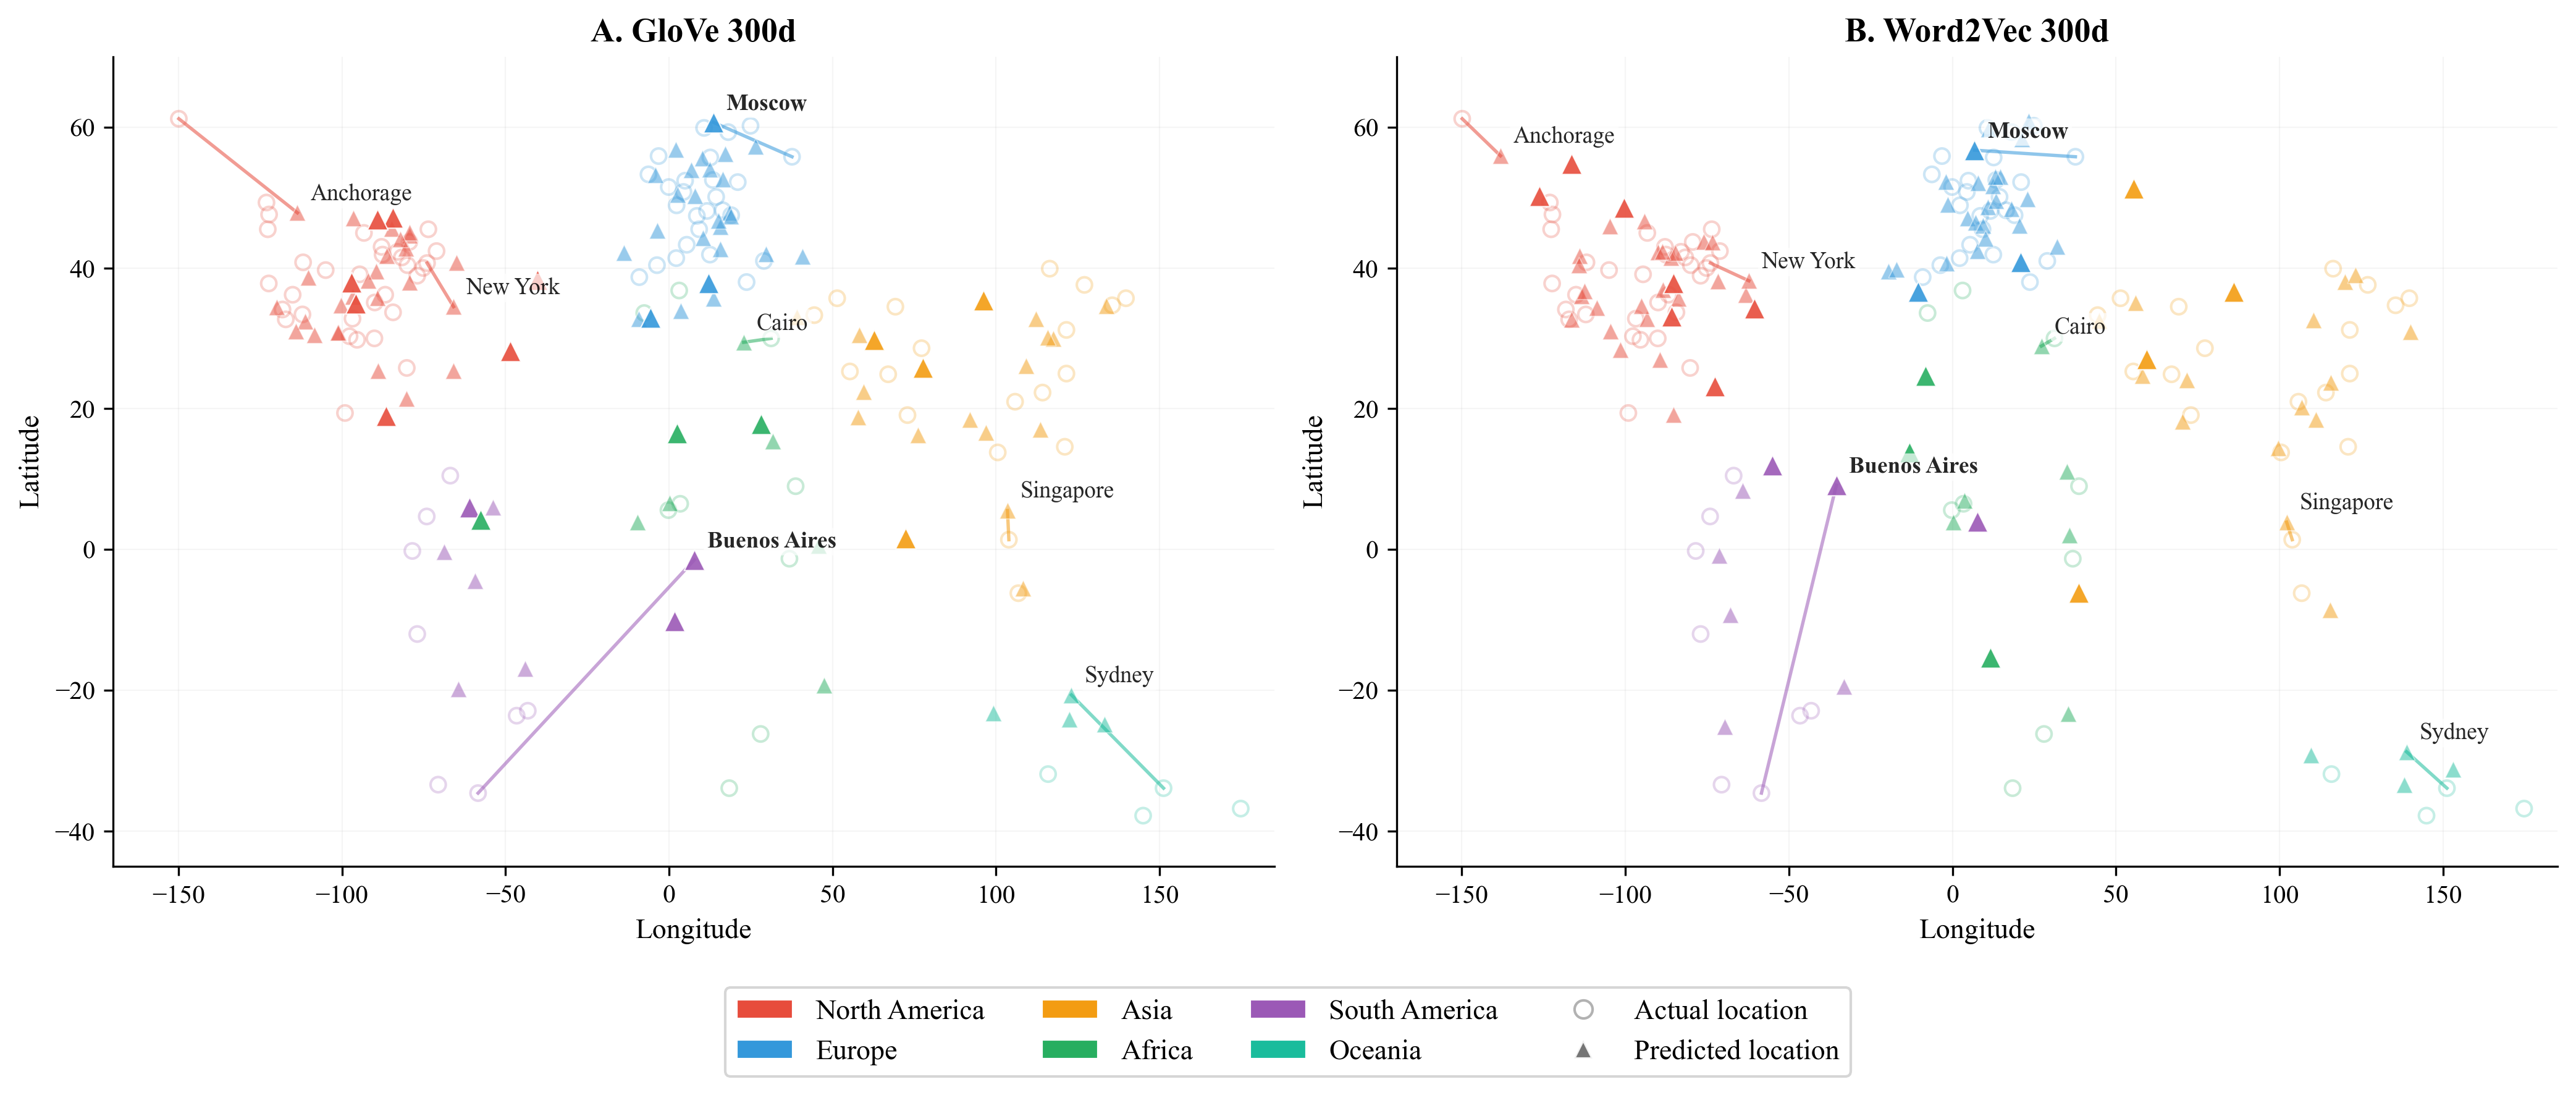
\includegraphics[width=\textwidth]{fig1_v1_overlay.png}
  \caption{Actual (open circles) versus predicted (filled triangles) city locations from ridge regression probes on GloVe and Word2Vec embeddings for all 99 cities. Lines connect actual and predicted positions for seven labeled cities to illustrate typical prediction error. Both models recover the broad global geographic layout from 300-dimensional word vectors alone.}
  \label{fig:geography}
\end{figure}

\paragraph{Negative controls.}
Elevation, GDP, and population do not systematically structure co-occurrence patterns in text, and accordingly yield negative or near-zero test $R^2$ (Table~\ref{tab:world_results}).
This demonstrates that linear probes do not trivially extract arbitrary world properties from embeddings; they are selective for distributional gradients present in the corpus, providing evidence that positive results reflect genuine distributional structure rather than probe overfitting.

\paragraph{Comparison with Gurnee et al.}
\citet{gurnee2023language} report $R^2 = 0.91$ for world-city coordinates using Llama-2-70B (layer 50), compared to our $R^2 = 0.71$--$0.87$ for static embeddings.
Static embeddings achieve 60--85\% of the LLM's performance with no contextual processing, attention, or multi-layer representations.
The datasets differ substantially in scale: \citeauthor{gurnee2023language} use $\sim$39,000 entities versus our 100.
Importantly, this asymmetry works \emph{against} our result: larger training sets give the probe more data to fit, typically increasing $R^2$.
That comparable signal is recoverable with only 80 training cities and a 300-dimensional linear probe indicates that the underlying distributional gradients are strong enough to be detected even under data-limited conditions.

\subsection{Historical Figures}

Table~\ref{tab:temporal_results} reports temporal probe results.
Both GloVe and Word2Vec predict birth, death, and midlife year with $R^2 = 0.46$--$0.52$, roughly 55--62\% of the $R^2 = 0.84$ reported by \citet{gurnee2023language} for Llama-2.

\begin{table}[t]
  \centering
  \caption{Ridge regression probe $R^2$ (test set) for 194 historical figures.}
  \label{tab:temporal_results}
  \begin{tabular}{lcccc}
    \toprule
    Target & GloVe $R^2$ & GloVe MAE (yr) & W2V $R^2$ & W2V MAE (yr) \\
    \midrule
    Birth Year   & 0.484 & 356 & 0.521 & 338 \\
    Death Year   & 0.460 & 364 & 0.516 & 338 \\
    Midlife Year & 0.472 & 360 & 0.519 & 338 \\
    \bottomrule
  \end{tabular}
\end{table}

Figure~\ref{fig:temporal} shows actual versus predicted birth years. The probes capture the broad distinction between ancient (pre-500 CE), medieval (500--1400), and modern (post-1400) eras, though with substantial compression of the timeline---ancient figures are predicted too late, and modern figures slightly too early, consistent with a signal carried by era-associated vocabulary rather than precise dates.

\begin{figure}[t]
  \centering
  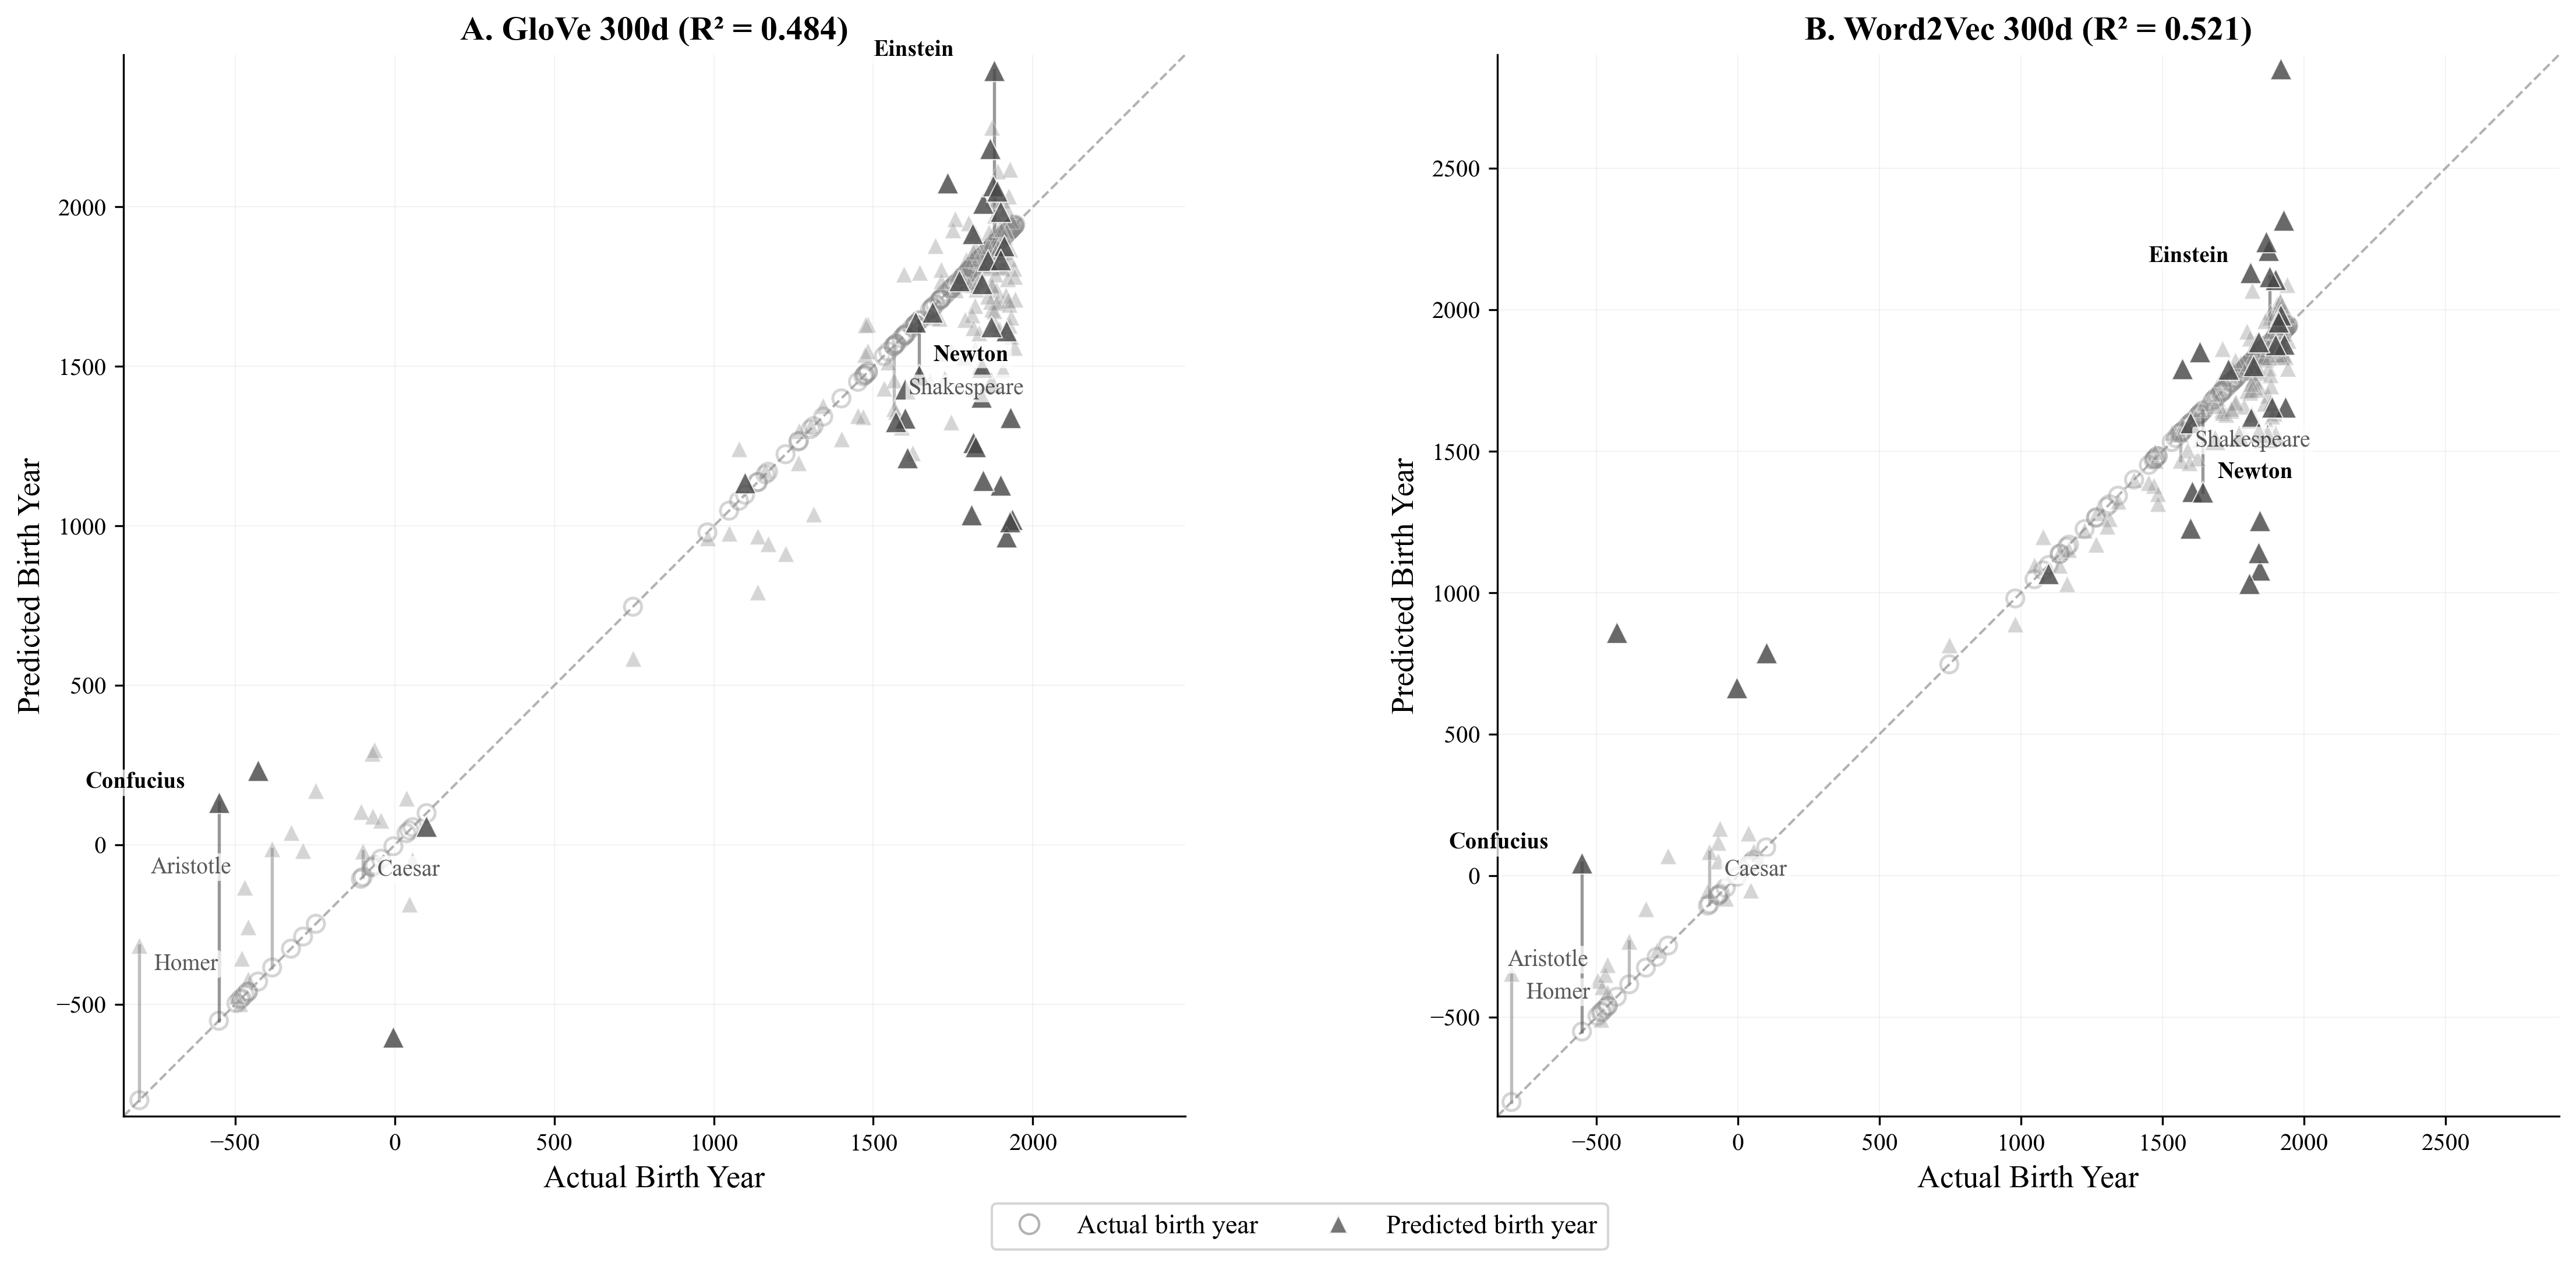
\includegraphics[width=\textwidth]{temporal_birth_year_scatter.png}
  \caption{Actual (open circles, on the diagonal) versus predicted (filled triangles) birth year for 194 historical figures. Lines connect actual and predicted values for labeled figures. The probe captures era-level temporal structure from both GloVe and Word2Vec embeddings.}
  \label{fig:temporal}
\end{figure}

\subsection{Semantic Similarity Analysis}

The preceding results establish that spatial and temporal targets are recoverable from static embeddings. We next ask whether this signal is interpretable: does the embedding space encode geography through co-occurrence with semantically meaningful vocabulary?

\paragraph{Individual word correlations.}
The cosine similarity between city embeddings and individual words correlates significantly with latitude and temperature (Figure~\ref{fig:semantic_spatial}).
Climate terms show the expected pattern: similarity to ``tropical'' correlates negatively with latitude ($r = -0.64$, $p < 0.001$), while similarity to ``frozen'' correlates positively ($r = +0.43$, $p < 0.001$).
Directional terms show similar patterns (``south'': $r = -0.43$), as do geopolitical terms reflecting the latitude-wealth correlation (``slum'': $r = -0.45$; ``chancellor'': $r = +0.42$).

A parallel pattern holds for temporal targets: similarity to ``ancient'' correlates with birth year at $r = -0.73$, ``greek'' at $r = -0.70$, and ``mythology'' at $r = -0.52$, identifying classical-era figures, while ``industrial'' and ``revolution'' mark later eras.

\begin{figure}[t]
  \centering
  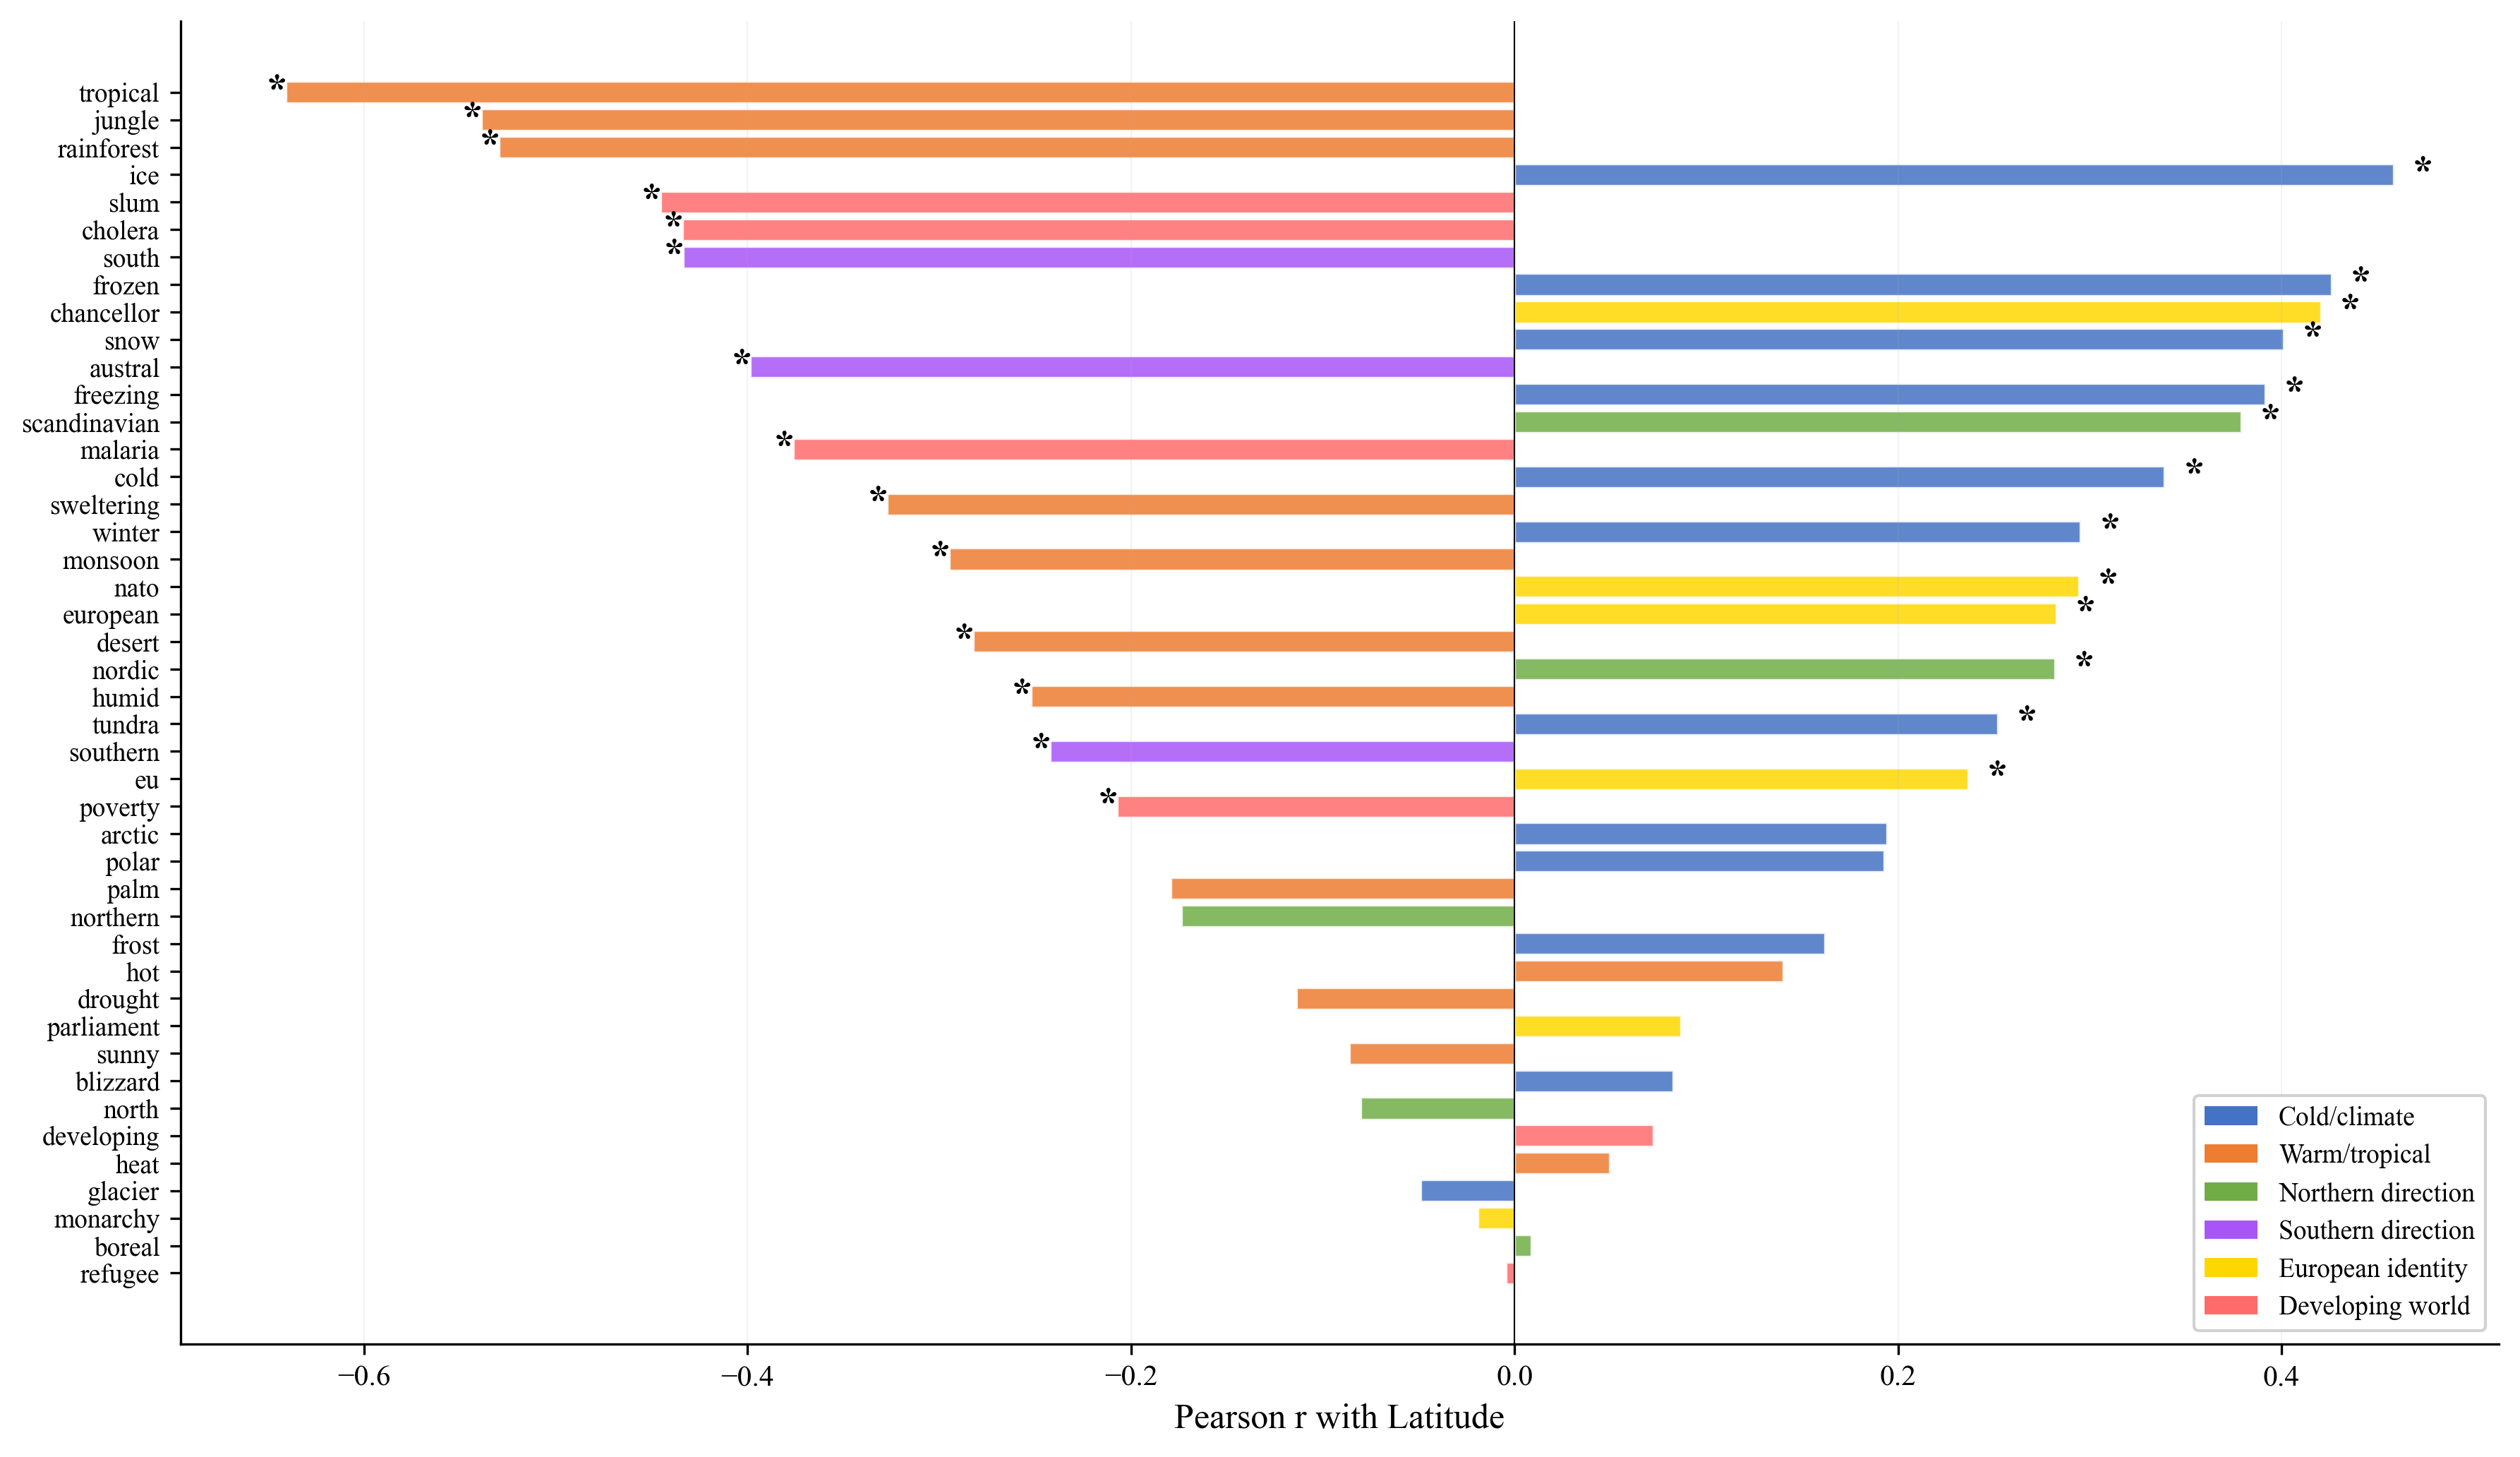
\includegraphics[width=0.85\textwidth]{semantic_word_lat_correlations.png}
  \caption{Pearson correlation between city--word cosine similarity and actual city latitude, for selected semantically meaningful words. Climate, directional, and geopolitical vocabulary all show significant correlations.}
  \label{fig:semantic_spatial}
\end{figure}

\paragraph{Composite scores.}
Composite scores constructed from antonym pairs provide strong continuous predictors.
The cold--warm composite (cosine similarity to ``cold'' minus similarity to ``warm'') correlates with latitude at $r = 0.61$ ($p < 0.0001$) and with temperature at $r = -0.79$ ($p < 0.0001$).
The modern--ancient composite correlates with birth year at $r = 0.63$ ($p < 0.0001$).
These results confirm that the probe signal is not opaque: it tracks interpretable co-occurrence structure that varies continuously with the target variables.


% ============================================================
% 5. DISCUSSION
% ============================================================
\section{Discussion}

\paragraph{Summary of findings.}
Across two widely used static embedding models (GloVe and Word2Vec), ridge regression probes predict geographic coordinates and historical dates from 300-dimensional vectors.
The same targets that have been used to motivate ``world model'' interpretations in LLMs are therefore linearly recoverable from representations that are explicit functions of global co-occurrence statistics and lack contextual processing.
Semantic similarity analyses confirm that this recoverability tracks interpretable co-occurrence structure.

\paragraph{Negative controls and probe selectivity.}
The negative controls in Table~\ref{tab:world_results} help delimit the scope of the effect.
While latitude, longitude, and temperature exhibit substantial signal, elevation, GDP per capita, and population do not.
This selectivity argues against an interpretation in which a linear probe acts as a general-purpose extractor of arbitrary world attributes.
Instead, recoverability tracks whether a target systematically structures co-occurrence patterns in text.

\paragraph{Explaining the performance gap.}
Static embeddings achieve roughly 60--85\% of the LLM's $R^2$ on world cities and 55--62\% on historical figures.
This gap does not necessitate a qualitative difference in representational mechanism.
Within a distributional account, LLMs have at least three systematic advantages: (i) contextual disambiguation (e.g., distinguishing ``Paris, France'' from ``Paris Hilton''); (ii) exposure to substantially larger corpora, yielding richer co-occurrence structure; and (iii) higher-dimensional intermediate representations that can preserve finer-grained distinctions.
Together, these factors can account for improved probe performance without requiring probe-based results to be interpreted as evidence for explicit internal world models.

\paragraph{Interpreting the signal.}
The semantic similarity analyses show that geographic recoverability tracks co-occurrence with vocabularies that correlate with location (e.g., climate descriptors, directional terms, and geopolitical references).
This provides a concrete pathway by which world-indexed variables can be linearly predictable from distributional representations: location covaries with stable lexical environments, which produce systematic structure in embedding space.

\paragraph{Implications for world-model claims.}
A prominent line of argument for emergent ``world models'' in large language models has relied on the linear recoverability of structured spatial and temporal properties from hidden states \citep[e.g.,][]{gurnee2023language, li2021implicit, patel2022mapping}.
The inference typically proceeds from decodability to structured internal representation.

Our results constrain this inference.
Because the same class of spatial and temporal signals is recoverable from static word embeddings that are direct functions of co-occurrence statistics, linear decodability alone cannot distinguish between structured internal modeling and inherited distributional gradients.
The observed recoverability is consistent with graded co-occurrence structure and does not, by itself, require contextual reasoning, attention mechanisms, or multi-layer computation.

This does not rule out the possibility that large language models construct structured representations of space or time.
Rather, it shows that probe-based recoverability, by itself, is insufficient evidence for that conclusion.
Claims of emergent world models must therefore demonstrate spatial or temporal resolution, compositional structure, or generalization behavior that exceeds what is recoverable from distributional baselines.

By Occam's razor, when a simpler mechanism---co-occurrence statistics---accounts for the observed signal, positing a more complex representational explanation requires additional empirical justification.

\paragraph{Limitations.}
Our results establish that spatial and temporal signals are recoverable from static co-occurrence-based embeddings.
However, this does not imply that large language models lack structured internal representations of space or time.
It shows only that linear decodability of such properties is not sufficient evidence for emergent world models.

First, our datasets are small relative to those used by \citet{gurnee2023language}.
While the persistence of substantial signal under these conditions suggests robustness rather than fragility---with limited training points and low-dimensional static embeddings, generalization is statistically harder---we cannot directly calibrate performance at scale.
Larger datasets may reveal systematic differences in how precisely spatial and temporal structure is encoded.

Second, static embeddings represent a lower bound on what distributional statistics can capture.
Contextual models trained on larger corpora may encode finer-grained or more compositional information not present in 300-dimensional word vectors.
Our results do not rule out the possibility that LLMs construct additional structure beyond distributional gradients.

Third, our analysis focuses on linear accessibility of information.
It remains possible that LLMs represent spatial or temporal structure in nonlinear forms not recoverable from static embeddings.
Demonstrating such differences would require tasks or probes that exceed what co-occurrence statistics alone can support.


% ============================================================
% 6. CONCLUSION
% ============================================================
\section{Conclusion}

We demonstrate that static word embeddings support linear recovery of geographic coordinates, temperature, and historical dates.
The recovered signal is interpretable: cosine similarity to climate, directional, and geopolitical vocabulary correlates systematically with geographic and temporal targets, confirming that the probe exploits semantically meaningful co-occurrence structure.

These findings reframe the interpretation of \citet{gurnee2023language}'s influential result.
The spatial and temporal structure they found in Llama-2 need not reflect emergent ``world models'' learned through next-word prediction; it may instead reflect the same distributional statistics that are explicitly captured by GloVe's co-occurrence matrix.
LLMs are better at recovering this information---likely due to contextual disambiguation and richer representations---but the qualitative nature of the signal appears to be the same.

More broadly, our findings underscore a methodological principle: linear decodability of structured world properties does not uniquely diagnose structured world modeling.
Distributional semantics alone can generate gradients that mimic spatial and temporal structure.
Before attributing emergent world models to language systems, it is necessary to rule out what co-occurrence statistics already provide.
``You shall know a word by the company it keeps'' \citep{firth1957synopsis} may explain more than is sometimes appreciated.


\paragraph{Reproducibility.}
All code and data (excluding pre-trained embedding files) are available at \url{https://github.com/elanbarenholtz/static-embeddings-space-time}.

% ============================================================
% REFERENCES
% ============================================================
\bibliographystyle{plainnat}
\bibliography{references}

\end{document}
